\documentclass[tikz,border=5pt]{standalone}
\usepackage[T1]{fontenc}
\usepackage{lmodern,amsmath,amssymb}
\usetikzlibrary{arrows.meta,calc,positioning,fit,backgrounds,shapes.geometric,matrix,decorations.pathreplacing,patterns}
\definecolor{ink}{gray}{0.08}
\definecolor{wash}{gray}{0.965}
\definecolor{soft}{gray}{0.45}
\tikzset{box/.style={draw=ink,line width=.65pt,fill=white,align=center,inner sep=4pt,outer sep=0pt,font=\small},flow/.style={draw=ink,line width=.65pt,-{Latex[length=1.8mm,width=1.3mm]},rounded corners=2pt},annotation/.style={font=\scriptsize,text=soft,align=center},groupbox/.style={draw=soft,dashed,line width=.45pt,fill=wash}}
\begin{document}
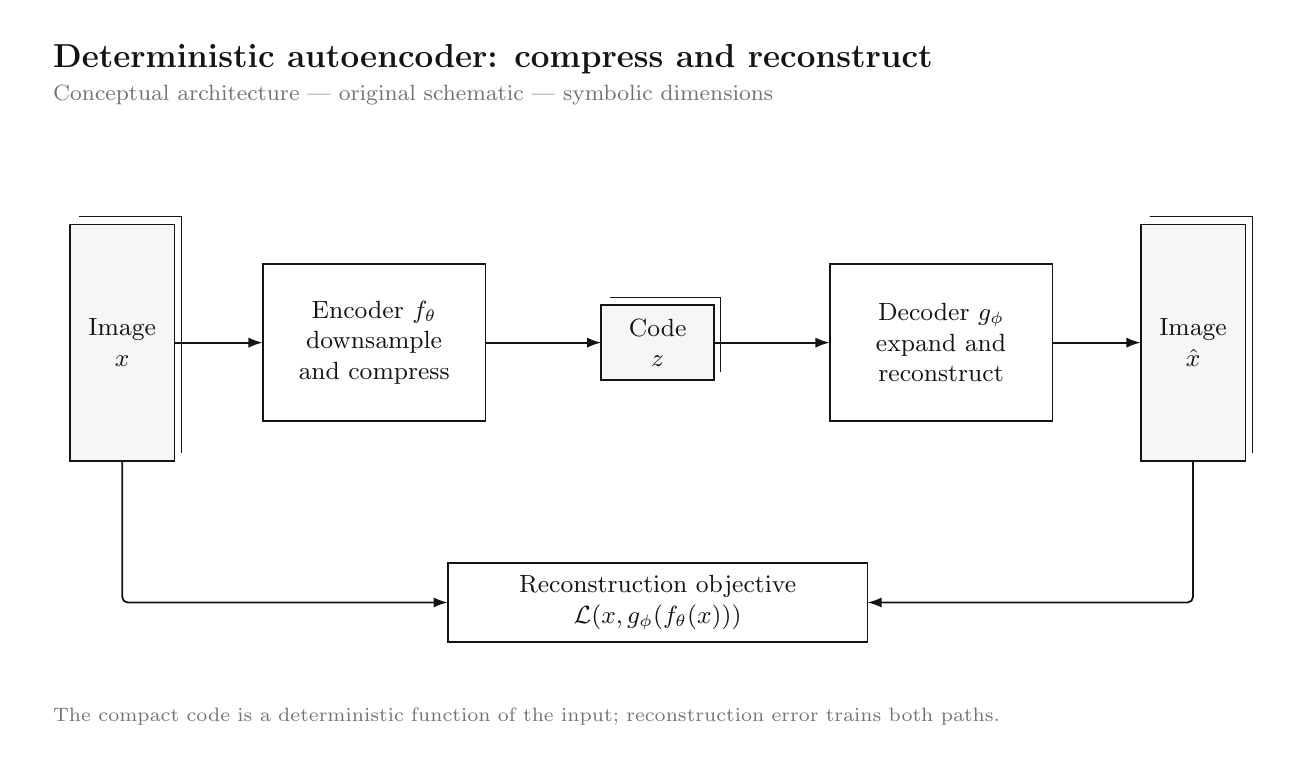
\begin{tikzpicture}[x=1cm,y=-1cm,font=\rmfamily,text=ink]

\path[use as bounding box] (0,0) rectangle (16,9);
\node[anchor=west,font=\large\bfseries] at (.2,.4) {Deterministic autoencoder: compress and reconstruct};
\node[anchor=west,font=\footnotesize,text=soft] at (.2,.85) {Conceptual architecture | original schematic | symbolic dimensions};
\begin{pgfonlayer}{background}
\end{pgfonlayer}
\node[box,fill=wash,minimum width=1.3cm,minimum height=3.0cm,text width=1.05cm] (x) at (1.2,4.0) {Image\\$x$};
\draw[ink,line width=.4pt] (0.6499999999999999,2.4) -- (1.9500000000000002,2.4) -- (1.9500000000000002,5.4);
\node[box,minimum width=2.8cm,minimum height=2.0cm,text width=2.55cm] (enc) at (4.4,4.0) {Encoder $f_\theta$\\downsample\\and compress};
\node[box,fill=wash,minimum width=1.4cm,minimum height=0.95cm,text width=1.15cm] (z) at (8.0,4.0) {Code\\$z$};
\draw[ink,line width=.4pt] (7.3999999999999995,3.425) -- (8.799999999999999,3.425) -- (8.799999999999999,4.375);
\node[box,minimum width=2.8cm,minimum height=2.0cm,text width=2.55cm] (dec) at (11.6,4.0) {Decoder $g_\phi$\\expand and\\reconstruct};
\node[box,fill=wash,minimum width=1.3cm,minimum height=3.0cm,text width=1.05cm] (xh) at (14.8,4.0) {Image\\$\hat x$};
\draw[ink,line width=.4pt] (14.25,2.4) -- (15.55,2.4) -- (15.55,5.4);
\node[box,minimum width=5.3cm,minimum height=1.0cm,text width=5.05cm] (loss) at (8.0,7.3) {Reconstruction objective\\$\mathcal L(x,g_\phi(f_\theta(x)))$};
\begin{pgfonlayer}{background}
\draw[flow] (x.east) -- (enc.west);
\draw[flow] (enc.east) -- (z.west);
\draw[flow] (z.east) -- (dec.west);
\draw[flow] (dec.east) -- (xh.west);
\draw[flow] (x.south) -- (1.2,7.3) -- (loss.west);
\draw[flow] (xh.south) -- (14.8,7.3) -- (loss.east);
\end{pgfonlayer}
\node[anchor=west,align=left,font=\scriptsize,text=soft,text width=15.6cm] at (.2,8.75) {The compact code is a deterministic function of the input; reconstruction error trains both paths.};
\end{tikzpicture}
\end{document}
